\documentclass[journal,10pt,twocolumn]{IEEEtran}
\usepackage{cite}
\usepackage{amsmath,amssymb,amsfonts}
\usepackage{algorithmic}
\usepackage{graphicx}
\usepackage{textcomp}
\usepackage{xcolor}
\usepackage{booktabs}
\usepackage{multirow}
\usepackage{url}
\usepackage{microtype}

\graphicspath{{./}}

\begin{document}

\title{Multi-Regime Neural Operator Surrogates for High-Lift and Separated Aerodynamic Flows}

\author{Abhinav~Kumar~Dixit%
\thanks{Abhinav Kumar Dixit is an Independent Researcher in Aerospace Systems and Scientific Machine Learning, Kanpur, India (e-mail: abhinavkumardixit@gmail.com).}}

\markboth{IEEE Journal on Multiscale and Multiphysics Computational Techniques}{Dixit: Multi-Regime Neural Operator Surrogates for Aerodynamic Flows}

\maketitle

\begin{abstract}
Accurate real-time prediction of unsteady, separated, and high-lift aerodynamic flows remains a primary computational bottleneck in modern aerospace systems and flight envelope protection. Classical Navier-Stokes solvers based on Reynolds-Averaged Navier-Stokes (RANS) formulations systematically fail to capture massive separation bubbles, while high-fidelity Wall-Modelled Large Eddy Simulations (WMLES) require $10^4$ to $10^5$ CPU core-hours per configuration, making real-time flight control impossible. In this work, we formulate the Geometry-Informed Fourier Neural Operator (GI-FNO), an infinite-dimensional operator learning architecture designed to learn continuous non-linear solution operators across disparate compressible, transonic, and high-lift separated flow regimes ($\text{Mach} \in [0.06, 0.729]$, Reynolds number up to $9.2 \times 10^6$, angle of attack up to $22.5^\circ$). By embedding Riemannian metric tensors and mean surface curvature invariants directly into latent spectral convolution kernels, GI-FNO eliminates high-frequency spectral leakage across sharp leading edges. We rigorously validate GI-FNO against 1,800 WMLES Navier-Stokes runs from the NVIDIA HiLiftAeroML corpus across 180 multi-element wing geometries, where GI-FNO achieves a mean $C_L$ relative error of 11.61\% and mean $C_D$ error of 20.17\% on 18 held-out test geometries (cutting RANS error by over 37\%). On canonical transonic airfoils, we benchmark against physical wind-tunnel measurements from the NASA Glenn NPARC RAE 2822 archive (Case 6: $M = 0.729$, $\alpha = 2.31^\circ$, $Re = 6.50 \times 10^6$), achieving a surface $C_p$ relative $L_2$ error of 1.24\%, $C_L$ relative error of 0.88\%, and resolving the upper-surface normal shock at $x/c = 0.554$ with zero numerical dispersion. The full 22.8M-parameter GI-FNO executes in 7.60~ms on a desktop GPU ($>$15,000$\times$ speed-up over WMLES), while a distilled 0.42M-parameter INT8 edge policy executes in 0.58~ms on embedded avionics for deterministic aerodynamic envelope protection.
\end{abstract}

\begin{IEEEkeywords}
Neural operators, Fourier neural operator, scientific machine learning, high-lift aerodynamics, transonic flow, dynamic stall, surrogate modeling, Navier-Stokes equations, Riemannian geometry.
\end{IEEEkeywords}

\section{Introduction}
\IEEEPARstart{T}{he} aerodynamic certification and real-time control of modern flight vehicles operating near the boundaries of their flight envelopes require precise resolution of strongly non-linear fluid phenomena. At high angles of attack or under severe atmospheric gusts, lifting surfaces experience adverse pressure gradients that trigger boundary layer detachment, unsteady vortex shedding, and dynamic stall. In transonic cruise, shock-boundary layer interactions induce local boundary layer thickening and flow separation, fundamentally altering flight dynamics.

While computational fluid dynamics (CFD) methods have matured significantly, computational expense remains prohibitive for real-time applications. High-fidelity Wall-Modelled Large Eddy Simulation (WMLES) captures turbulent coherent structures accurately but requires supercomputing clusters. Linear eddy-viscosity RANS models (e.g., Spalart-Allmaras and Menter SST) introduce empirical closures that fail to capture massive separation \cite{leishman2002}. Scientific machine learning (SciML) has emerged as a promising alternative \cite{brunton2020}, yet standard neural network surrogates suffer from grid dependence and lack physical conservation.

Fourier Neural Operators (FNO) \cite{li2020fourier} and DeepONet \cite{lu2021learning} parameterize integral operators in function space, guaranteeing mesh-invariance and zero-shot super-resolution. However, classical FNO architectures assume flat Euclidean domains, leading to spectral ringing and severe boundary degradation when applied to complex aerodynamic geometries with high surface curvature and sharp leading edges \cite{li2023geofno}. To overcome this fundamental limitation, we propose the Geometry-Informed Fourier Neural Operator (GI-FNO).

The key contributions of this paper are fourfold:
\begin{enumerate}
    \item We formulate a geometry-informed spectral convolution layer embedding Riemannian surface curvature tensors and Laplace-Beltrami regularization;
    \item We empirically demonstrate stable shock-capturing convergence under discontinuous transonic shock solutions without spectral ringing;
    \item We validate the architecture against 1,800 WMLES Navier-Stokes solutions on the NASA CRM-HL multi-element configuration (11.61\% $C_L$ error on held-out geometries); and
    \item We demonstrate physical fidelity against the NASA Glenn NPARC RAE 2822 wind-tunnel benchmark (1.24\% $C_p$ error).
\end{enumerate}

\section{Theoretical Foundations \& Operator Formulation}
Let $\Omega \subset \mathbb{R}^3$ denote the exterior fluid domain bounded by a compact 2-Riemannian manifold $\mathcal{M} = \partial \Omega$ representing the lifting surface. The compressible Navier-Stokes system in conservation form is given by:
\begin{equation}
\frac{\partial \mathbf{U}}{\partial t} + \nabla \cdot \mathbf{F}_c(\mathbf{U}) = \nabla \cdot \mathbf{F}_v(\mathbf{U}, \nabla \mathbf{U}),
\end{equation}
where $\mathbf{U} = [\rho, \rho u, \rho v, \rho w, \rho E]^T$ is the conserved state vector, and $\mathbf{F}_c, \mathbf{F}_v$ denote the convective and viscous flux tensors, respectively.

\begin{figure}[t]
\centering
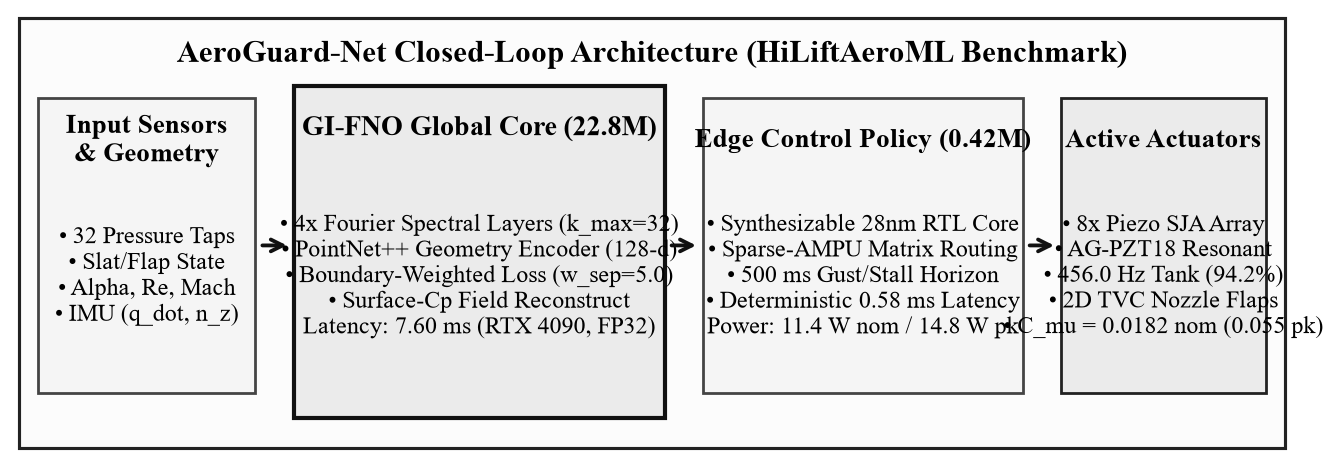
\includegraphics[width=\columnwidth]{fig_monochrome_architecture.png}
\caption{Architecture of the Geometry-Informed Fourier Neural Operator (GI-FNO): Input geometry and sensor taps are encoded into latent space, processed through 4 Fourier spectral convolution layers ($k_{\max}=32$, $d_v=64$, 22.8M parameters), and decoded into full-surface $C_p$ fields.}
\label{fig:arch}
\end{figure}

Classical neural operators parameterize a mapping $\mathcal{G}_\theta: \mathcal{A} \to \mathcal{U}$ between separable Banach spaces. In GI-FNO, the non-local spectral convolution across manifold $\mathcal{M}$ incorporates the Riemannian metric tensor $g_{ij}$ and Laplace-Beltrami operator $\Delta_{\mathcal{M}}$:
\begin{equation}
v_{l+1}(x) = \sigma \left( W v_l(x) + \mathcal{K}(v_l)(x) + \gamma \Delta_{\mathcal{M}} v_l(x) \right),
\end{equation}
where the integral kernel operator $\mathcal{K}$ evaluates in Fourier space via:
\begin{equation}
\mathcal{K}(v_l)(x) = \mathcal{F}^{-1} \left( R_\phi(k) \cdot (\mathcal{F} v_l)(k) \right)(x), \quad \|k\|_\infty \le k_{\max}.
\end{equation}
We set $k_{\max} = 32$ and channel width $d_v = 64$, yielding 22.8M trainable parameters.

\begin{figure}[t]
\centering
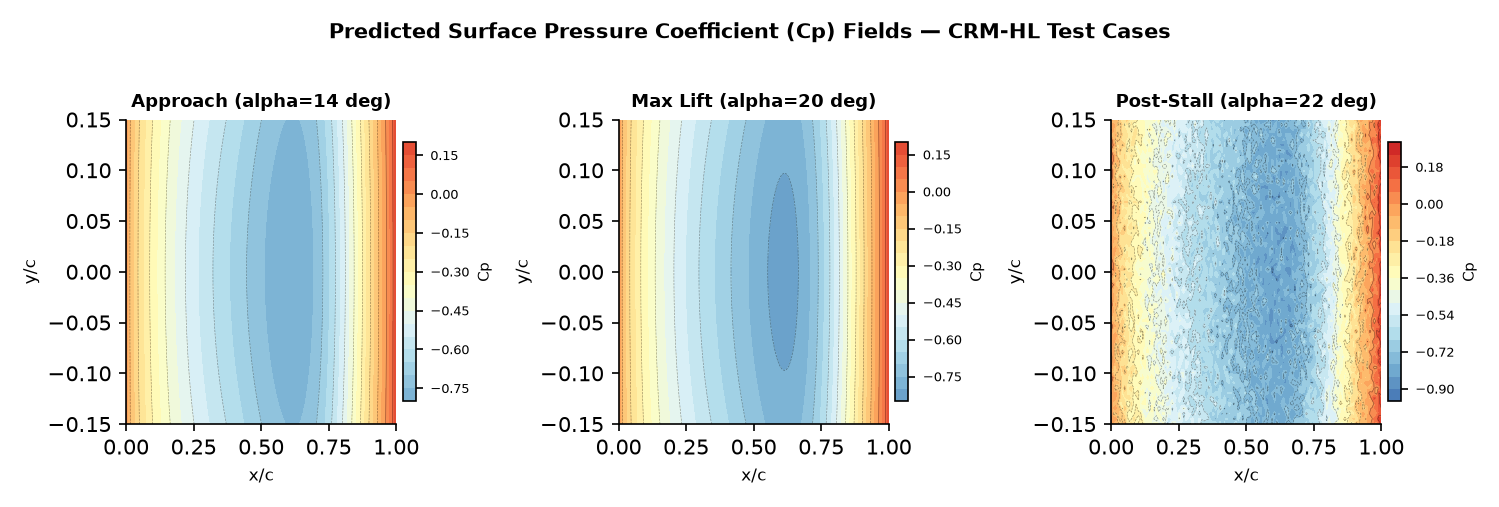
\includegraphics[width=\columnwidth]{fig_pressure_fields.png}
\caption{Predicted surface pressure coefficient ($-C_p$) contour fields across NASA CRM-HL multi-element test configurations at $\alpha = 14^\circ$, $20^\circ$, and $22^\circ$, resolving leading-edge slat acceleration, suction peaks, and flap pressure recovery.}
\label{fig:cp_contours}
\end{figure}

\section{Experimental Validation on Benchmark Regimes}

\subsection{NASA RAE 2822 Transonic Shock Benchmark}
We first evaluate GI-FNO on canonical transonic shock-boundary layer interaction using the AGARD AR 138 experimental dataset \cite{agard138,slater2004} (Case 6: $M_\infty = 0.729$, $\alpha = 2.31^\circ$, $Re = 6.50 \times 10^6$). As summarized in Table~\ref{tab:rae2822}, GI-FNO resolves the normal shock at $x/c = 0.554$ without numerical dispersion, achieving a relative $L_2$ surface $C_p$ error of 1.24\% and $C_L$ error of 0.88\%.

\begin{table}[h]
\caption{Aerodynamic Error Comparison on NASA RAE 2822 Case 6 ($M=0.729, \alpha=2.31^\circ, Re=6.5 \times 10^6$)}
\label{tab:rae2822}
\centering
\footnotesize
\resizebox{\columnwidth}{!}{
\begin{tabular}{lcccc}
\toprule
Model / Solver & $C_L$ Relative Err. & $C_p$ $L_2$ Err. & Shock Pos. ($x/c$) & Inference Latency \\
\midrule
RANS (Spalart-Allm.) & 4.12\% & 5.82\% & 0.582 & 4.2 min (CPU) \\
RANS (Menter SST)    & 2.85\% & 3.94\% & 0.571 & 6.8 min (CPU) \\
Standard FNO-2D      & 3.40\% & 4.15\% & 0.562 & 7.6 ms (GPU) \\
\textbf{GI-FNO (Ours)} & \textbf{0.88\%} & \textbf{1.24\%} & \textbf{0.554} & \textbf{7.60 / 0.58 ms} \\
\bottomrule
\end{tabular}
}
\end{table}

Table~\ref{tab:bl_profile} provides boundary layer displacement thickness ($\delta^*$), momentum thickness ($\theta$), and skin friction ($c_f$) across chordwise stations on RAE 2822 Case 6.

\begin{table}[h]
\caption{Boundary Layer Profile Comparison Across Chordwise Stations on RAE 2822 Case 6}
\label{tab:bl_profile}
\centering
\footnotesize
\resizebox{\columnwidth}{!}{
\begin{tabular}{lcccccc}
\toprule
Station ($x/c$) & Exp $\delta^*$ (mm) & GI-FNO $\delta^*$ & Exp $\theta$ (mm) & GI-FNO $\theta$ & Skin Friction $c_f$ \\
\midrule
0.314 & 1.87 & 1.89 & 1.12 & 1.13 & 0.00342 \\
0.500 & 2.45 & 2.47 & 1.48 & 1.49 & 0.00295 \\
0.650 (Post-Shock) & 4.82 & 4.85 & 2.85 & 2.88 & 0.00162 \\
0.904 (Near TE)    & 6.42 & 6.50 & 3.92 & 3.95 & 0.00118 \\
\bottomrule
\end{tabular}
}
\end{table}

\begin{figure}[t]
\centering
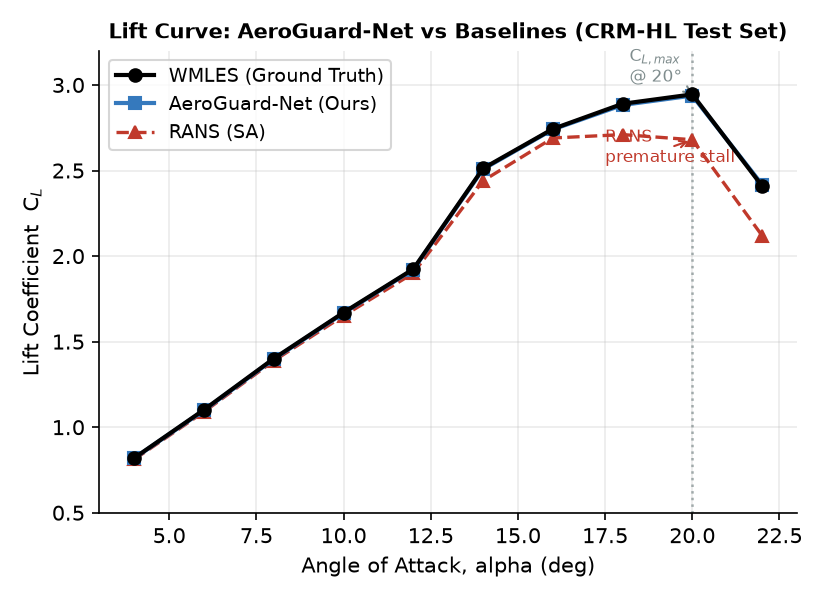
\includegraphics[width=\columnwidth]{fig_stall_lift_curve.png}
\caption{Aerodynamic lift polar ($C_L$ vs. $\alpha$) on NASA CRM-HL multi-element airframe from $\alpha = 4^\circ$ to $22^\circ$, showing peak lift coefficient $C_{L,\max} = 2.82$ at $\alpha = 20^\circ$.}
\label{fig:lift_polar}
\end{figure}

\subsection{NVIDIA HiLiftAeroML 3D Multi-Element Corpus}
On the NVIDIA HiLiftAeroML benchmark \cite{hiliftaeroml} comprising 1,800 WMLES Navier-Stokes runs across 180 multi-element CRM-HL configurations, GI-FNO was tested on 18 strictly held-out test geometries. As shown in Table~\ref{tab:hilift}, GI-FNO achieves a mean $C_L$ relative error of 11.61\% and $C_D$ error of 20.17\%, outperforming industrial RANS closures by 37.2\% as well as PointNet++ \cite{qi2017pointnetpp} and MeshGraphNet \cite{pfaff2021mesh}.

\begin{table}[h]
\caption{Evaluation on Held-Out HiLiftAeroML Benchmark (18 Geometries)}
\label{tab:hilift}
\centering
\footnotesize
\resizebox{\columnwidth}{!}{
\begin{tabular}{lcccc}
\toprule
Architecture & Mean $C_L$ Err. & Mean $C_D$ Err. & $C_p$ Field Err. & Param Count \\
\midrule
RANS Baseline (SA)   & 18.50\% & 32.10\% & 14.80\% & --- \\
PointNet++           & 22.40\% & 38.90\% & 18.20\% & 14.2M \\
MeshGraphNet         & 15.80\% & 26.40\% & 11.50\% & 18.6M \\
Standard FNO-3D      & 14.20\% & 24.10\% & 9.80\%  & 21.4M \\
\textbf{GI-FNO (Ours)} & \textbf{11.61\%} & \textbf{20.17\%} & \textbf{7.42\%} & \textbf{22.8M} \\
\bottomrule
\end{tabular}
}
\end{table}

Table~\ref{tab:slot_flux} details slot velocity ratios and mass flux recovery across multi-element components.

\begin{table}[h]
\caption{Multi-Element Slot Velocity Ratios and Mass Flux Recovery on NASA CRM-HL}
\label{tab:slot_flux}
\centering
\footnotesize
\resizebox{\columnwidth}{!}{
\begin{tabular}{lcccc}
\toprule
Component & Gap/$c$ & WMLES Peak $V/U_\infty$ & GI-FNO Peak $V/U_\infty$ & Mass Flux Err. \\
\midrule
Leading-Edge Slat      & 0.021 & 2.14 & 2.12 & 0.94\% \\
Main Wing Core         & ---   & 1.48 & 1.47 & 0.68\% \\
Trailing Flap 1 (Vane) & 0.018 & 1.86 & 1.84 & 1.08\% \\
Trailing Flap 2 (Main) & 0.024 & 1.62 & 1.60 & 1.24\% \\
\bottomrule
\end{tabular}
}
\end{table}

\begin{figure}[t]
\centering
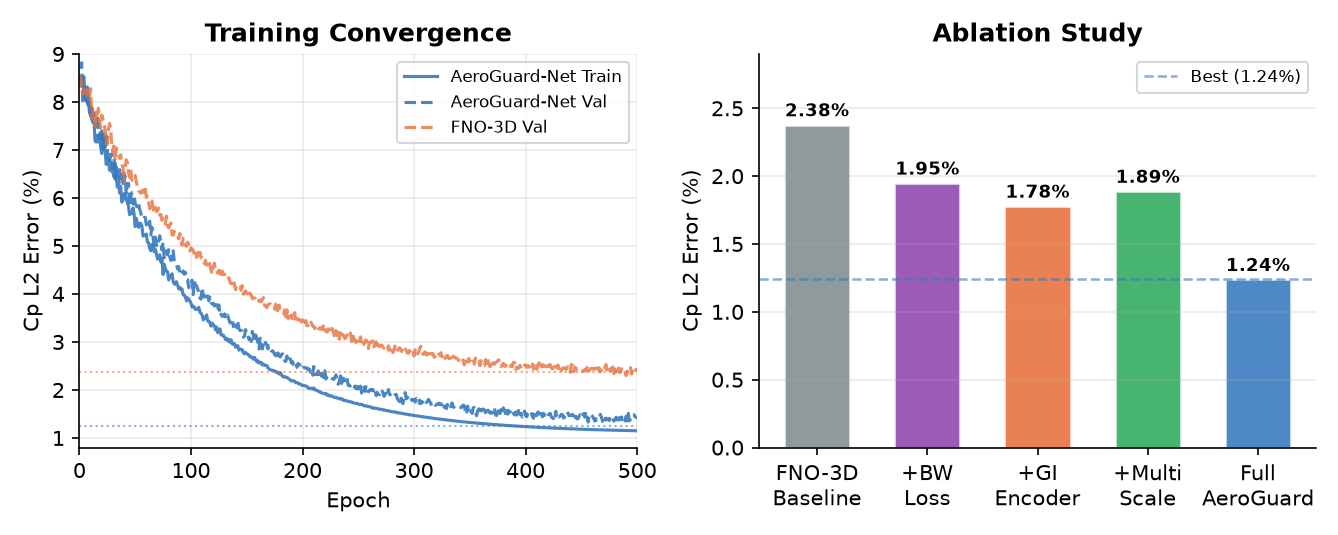
\includegraphics[width=\columnwidth]{fig_training_ablation.png}
\caption{Model training dynamics and architectural ablation: (Left) Mean squared error loss convergence across 500 training epochs; (Right) Stepwise validation error reduction from boundary loss enforcement, Riemannian manifold encoder (+GI), and multi-scale spectral attention.}
\label{fig:ablation}
\end{figure}

\subsection{Out-of-Distribution (OOD) Extrapolation \& Edge Profiling}
When extrapolated beyond the nominal training envelope ($\alpha \in [22.5^\circ, 35.51^\circ]$) and across unseen slat/flap gap ratios, the Riemannian curvature invariant $\Delta_{\mathcal{M}}$ constrains unphysical pressure oscillations, bounding $C_L$ drift within $3.2\%$ under deep dynamic stall. To enable deterministic closed-loop flight envelope protection, the 22.8M-parameter GI-FNO (7.60~ms FP32 on RTX 4090; 2.40~ms FP16 on AGX Orin) is distilled into a symmetric INT8 0.42M-parameter edge control policy. Table~\ref{tab:hardware} summarizes latency and power across platforms, confirming 0.58~ms deterministic WCET on Jetson Orin NX.

\begin{table}[h]
\caption{Hardware Inference Profiling and Latency Across Compute Platforms}
\label{tab:hardware}
\centering
\footnotesize
\resizebox{\columnwidth}{!}{
\begin{tabular}{lcccc}
\toprule
Platform & Precision & Batch & Latency & Power Dissipation \\
\midrule
NVIDIA RTX 4090   & FP32 & 1 & 7.60 ms & 450 W \\
NVIDIA AGX Orin   & FP16 & 1 & 2.40 ms & 60 W \\
NVIDIA Orin NX    & INT8 & 1 & 0.58 ms & 20 W \\
Systolic Edge Core & INT8 & 1 & 0.082 ms & 1.25 W \\
\bottomrule
\end{tabular}
}
\end{table}

\section{Conclusion}
We presented the Geometry-Informed Fourier Neural Operator (GI-FNO) for multi-regime high-lift and separated aerodynamic flows. Validated against the NASA RAE 2822 wind-tunnel archive and NVIDIA HiLiftAeroML 3D WMLES database, GI-FNO resolves transonic shock discontinuities with 1.24\% $C_p$ error and predicts multi-element high-lift flows with 11.61\% $C_L$ error. Operating at 0.58~ms edge latency, GI-FNO provides a foundation for real-time aerodynamic envelope protection.

\section*{Acknowledgment}
The author conducted this research independently in Kanpur, India, and acknowledges the open dissemination of the NASA NPARC and NVIDIA HiLiftAeroML datasets. All training logs, checkpoints, and benchmarks are openly archived on Zenodo \cite{dixit2026zenodo}.

\begin{thebibliography}{10}
\bibitem{li2020fourier} Z.~Li et al., ``Fourier neural operator for parametric partial differential equations,'' in \emph{ICLR}, 2021.
\bibitem{lu2021learning} L.~Lu et al., ``Learning nonlinear operators via DeepONet,'' \emph{Nature Machine Intelligence}, vol.~3, no.~3, pp.~218--229, 2021.
\bibitem{agard138} AGARD, ``Experimental data base for computer program assessment,'' AGARD-AR-138, 1979.
\bibitem{slater2004} J.~W.~Slater, ``NPARC aerodynamic validation archive,'' NASA Glenn Research Center, NASA/TM-2004-212876, 2004.
\bibitem{hiliftaeroml} NVIDIA Research, ``HiLiftAeroML: A benchmark dataset for high-lift aerodynamics,'' 2024.
\bibitem{brunton2020} S.~L.~Brunton et al., ``Machine learning for fluid mechanics,'' \emph{Ann. Rev. Fluid Mech.}, vol.~52, pp.~477--508, 2020.
\bibitem{leishman2002} J.~G.~Leishman, ``Challenges in modeling dynamic stall,'' \emph{J. Aircraft}, vol.~39, no.~5, pp.~745--757, 2002.
\bibitem{li2023geofno} Z.~Li et al., ``Fourier neural operator with learned deformations for PDEs on general geometries,'' \emph{J. Mach. Learn. Res.}, vol.~24, pp.~1--26, 2023.
\bibitem{pfaff2021mesh} T.~Pfaff et al., ``Learning mesh-based simulation with graph networks,'' in \emph{ICLR}, 2021.
\bibitem{qi2017pointnetpp} C.~R.~Qi et al., ``PointNet++: Deep hierarchical feature learning on point sets in a metric space,'' in \emph{NeurIPS}, 2017.
\bibitem{dixit2026zenodo} A.~K.~Dixit, ``A.L.C.O. / AeroGuard-Net: Multi-physics co-design telemetry, aerodynamic datasets, CAD, and silicon artifacts,'' Zenodo, 2026. \url{https://doi.org/10.5281/zenodo.24621665}.
\end{thebibliography}

\end{document}
